\documentclass[11pt,a4paper,twocolumn]{article}

\usepackage[margin=1in]{geometry} 
\usepackage[utf8]{inputenc} 
\usepackage[T1]{fontenc} 
\usepackage{lmodern} 
\usepackage{sectsty} 
\usepackage{titlesec} 
\usepackage{fancyhdr}\usepackage{hyperref}
\usepackage{graphicx}
\usepackage{caption}
\usepackage{paralist}
\usepackage{tabularx}
\usepackage{tikz}
\usepackage{tgheros}

\usetikzlibrary{shapes,arrows,positioning}

% Section styles
\sectionfont{\large\bfseries}
\subsectionfont{\normalsize\bfseries}
\subsubsectionfont{\normalsize\itshape}
\renewcommand{\familydefault}{\sfdefault}

% Headers/Footers
\pagestyle{fancy}
\fancyhf{}
\lhead{MK-500 Crypto Unit}
\rhead{Rev A1.3}
\cfoot{\thepage}

% Title formatting
\titleformat{\section}{\large\bfseries}{\thesection.}{0.5em}{}
\titleformat{\subsection}{\normalsize\bfseries}{\thesubsection.}{0.5em}{}
\titleformat{\subsubsection}{\normalsize\itshape}{\thesubsubsection.}{0.5em}{}

% Hyperref setup
\hypersetup{ colorlinks=false, pdfborder={0 0 0}, pdftitle={MK-500 Crypto Unit Datasheet}, pdfauthor={MasterUpSkyTerminal Inc.}, pdfsubject={Embedded Device Specifications}, pdfkeywords={MK-500, RM-230, UXR-10, datasheet, embedded systems} }
\setlength{\columnsep}{0.35in}
\begin{document}
\begin{center} {\huge\textbf{MK-500 Crypto Unit for Satellite Communications}\\[0.5cm]} {\Large Datasheet (Revision A1.3)}\\[0.5cm] {\large Date: 2025-03-01}\\[0.5cm]
\textbf{Document Number:} DS-MK500-A1.3
\end{center}
\vspace{1cm}
\tableofcontents

\newpage

\section{Introduction} The MK-500 Crypto Unit for Satellite Communications is the latest satellite communication module by MasterUpSkyTerminal Inc. MK-500 is designed for use in advanced sensor systems that require secure, encrypted, low-latency communication, configurable firmware updates, and a modular user interface. The device is the core of a three-module system, including:

\begin{compactitem}
\item
\textbf{CM-500 Crypto Module}
\item
\textbf{RM-230 Radio Interface Module}
\item
\textbf{UXR-10 Interface Module}
\end{compactitem} 
MK-500 is specifically designed for use in space or satellite systems as the main communication device. Additionally, supporting components ensure stable power, memory operations, and signal integrity. This datasheet provides hardware-level details, interface specifications, and recommended operational parameters. Integration notes for firmware handling, including data integrity measures and proprietary modulation constants, are also included.

\section{System Overview}
\subsection{Block Diagram} Figure~\ref{fig:block_diagram} shows a schematic overview of the system. CM-500 forms the center, with RM-230 and UXR-10 interfaced over UART and other serial lines. RM-230 is responsible for sending and receiving encrypted signals to the external communication interfaces, CM-500 handles the main encryption and decryption of the messages and the interface module allow for a smooth connection interface to other external units.  

\begin{figure*}[t]
\centering
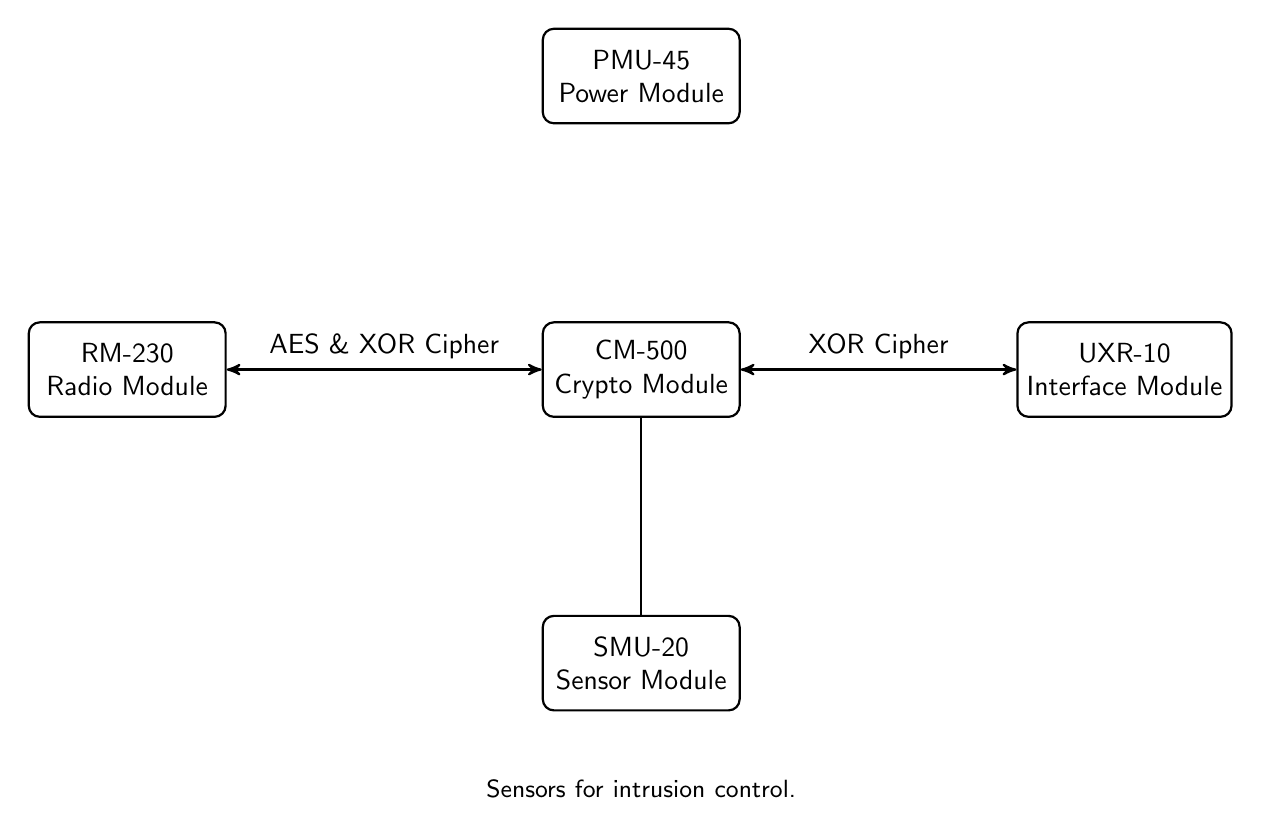
\begin{tikzpicture}[>=stealth', thick, node distance=2.5cm] % Styles
\tikzstyle{module}=[draw, thick, rounded corners, align=center, minimum width=2.5cm, minimum height=1.2cm]
\tikzstyle{data}=[draw, thick, rounded corners, align=center, fill=gray!20, minimum width=2.2cm, minimum height=1cm] % Nodes
\node[module] (mk500) {CM-500\\Crypto Module};
\node[module, left=of mk500, xshift=-1.5cm] (rim230) {RM-230\\Radio Module};
\node[module, right=of mk500, xshift=1.0cm] (uxr10) {UXR-10\\Interface Module};
\node[module, above=of mk500] (pmu45) {PMU-45\\Power Module};
\node[module, below=of mk500] (pll20) {SMU-20\\Sensor Module}; % Connections
\draw[<->] (rim230) -- node[above]{AES \& XOR Cipher} (mk500);
\draw[<->] (mk500) -- node[above]{XOR Cipher} (uxr10);
\draw (pll20) -- (mk500); % Additional labels
\node[align=center, below of=pll20, yshift=1.0cm, text width=7cm] {\small 

Sensors for intrusion control.};
\end{tikzpicture}
\caption{MK-500 system description. Plaintext is sent to and from UXR-10}
\label{fig:block_diagram}
\end{figure*}

\subsection{CM-500 Crypto} CM-500 serves as the central processor for the encryption and decryption of messages to and from RM-230. It runs the main crypto firmware, manages the configuration parameters, handling of encryption keys to and from secure storage and orchestrates data flows between peripheral modules. Key features:
\begin{compactitem}
\item 
\textbf{ARM\textsuperscript{\textregistered} Cortex\textsuperscript{\textregistered}-A5 Core:} 500 MHz.
\item
\textbf{Embedded SRAM
\& Flash NVM}
\item
\textbf{Secure storage:} Secure handling of keys.
\item
\textbf{High-Speed Serial Interfaces:} Connects to RM-230 and UXR-10.
\end{compactitem} 
The crypto module is responsible for encrypting and decrypting the demodulated messages from RM-230 with AES-128 CBC. The messages to and from UXR-10 however is not in pure plaintext since the communication between UXR-10 and CM-500 is protected by a XOR Cipher. This includes both the external messages and the internal debug messages going to and from UXR-10. In its standard configuration, the crypto in MK-500 uses a pre-defined encryption key stored in a secure memory in the device. This allow for an easy and secure setup between other MK-500 devices. 

CM-500 is also equipped with the latest protection mechanisms against unauthorized physical access. CM-500 checks, via the sensor module SMU-20, continuously for changes in the environment and proximity indicators for physical intruders trying to access the cryptographic module. If a physical intrusion is detected, the system restarts and thereby setting itself to a secure state without any plaintext data.  

\subsection{RM-230 Radio Interface Module} 
The RM-230 attaches via a serial interface to the MK-500. It receives and sends the encrypted messages. When sending messages it modulates the data in order to send it over a long range communication channel. When receiving data, it demodulates the signal and send it to CM-500. The data being sent to and from CM-500 is encrypted both with AES and the underlying XOR cipher.  

\subsection{UXR-10 Interface Module} The UXR-10 Interface Module provides a simple interface between the CM-500 and external systems:

\begin{compactitem}
\item Receives and sends fully decrypted plaintext messages after applying the internal XOR cipher.
\item Receives and sends messages with the XOR Cipher applied to/from CM-500 with LSB first over a serial interface (115200 baud, 8N1). All messages going on the channel between UXR-10 and CM-500 are therefore encrypted with the XOR Cipher. 
\end{compactitem}

\section{Additional Components}
\subsection{PMU-45 Power Module} The PMU-45 ensures stable voltage and is the interface to the external power supply. 
\subsection{SMU-20 Sensor Module} Acts as a interface between the sensors measuring environment and proximity indicators in order to indicate if a physical intrusion is taking place. If the sensors pick up a proximity indication, a signal will be sent to CM-500 to start the secure state process. 
\subsection{Debug Port and JTAG Access to CM-500} For troubleshooting of the crypto module CM-500, JTAG and debug UART ports are available. The UART debug interface allow for getting a shell by interrupting the startup process if connecting to the serial connector between the crypto module and the interface module. If not interrupting the startup process, debug logs will be available over the UART interface. Note that only debug tools from MasterUpSkyTerminal Inc can be used for this since the UART debug interface is protected by the XOR cipher. Since the debug line used is connected in parallel to the CM-500/UXR-10 interface, all communication between these devices can also be seen by connecting to the UART debug interface.

\section{Operational Considerations}
\subsection{Firmware Update Procedure}
Firmware updates of MK-500 are provided by MasterUpSkyTerminal Inc. For the update procedure, refer to the document Software Update Procedures (SU-MK500). 

\section{Recommended Handling and Safety}
\begin{compactitem}
\item Use official firmware images from trusted sources.
\item Do not place the device close to any pets. 
\end{compactitem}

\section{Revision History}
\begin{tabularx}{\linewidth}{lX}
\textbf{Rev} &
\textbf{Changes}
\\
\hline A1.3 & Clarified RM-230 operation and removed the standard XOR cipher key from the document for security reasons.
\\ A1.2 & Added buffering details for RM-230 and changed 0x42 to 0x67 as the updated standard key between the crypto module and the interface module.
\\ A1.0 & Initial release.
\\
\end{tabularx}
\vfill
\noindent
\textbf{End of Document}
\end{document}